\documentclass[tikz,border=7pt]{standalone}
\usepackage{amsmath}
\usepackage{pgfplots}
\usepgfplotslibrary{groupplots}
\pgfplotsset{compat=1.18}
\definecolor{ink}{HTML}{17324D}
\definecolor{accent}{HTML}{0F766E}
\definecolor{gold}{HTML}{C28524}
\begin{document}
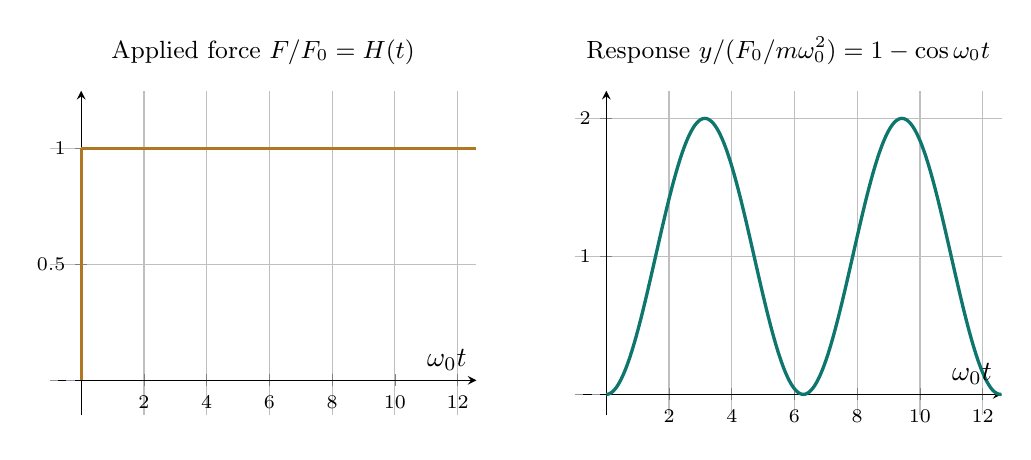
\begin{tikzpicture}
\begin{groupplot}[
 group style={group size=2 by 1,horizontal sep=1.25cm},
 width=7cm,height=5.7cm,
 xmin=-1,xmax=12.6,axis lines=middle,grid=both,
 tick label style={font=\scriptsize},title style={font=\small},
 xlabel={$\omega_0t$},
]
\nextgroupplot[title={Applied force $F/F_0=H(t)$},ymin=-.15,ymax=1.25]
 \addplot[ink!50,dashed,domain=-1:0,samples=2]{0};
 \addplot[gold!90!black,very thick,domain=0:12.6,samples=2]{1};
 \draw[gold!90!black,very thick] (axis cs:0,0)--(axis cs:0,1);
\nextgroupplot[title={Response $y/(F_0/m\omega_0^2)=1-\cos\omega_0t$},ymin=-.15,ymax=2.2]
 \addplot[ink!50,dashed,domain=-1:0,samples=2]{0};
 \addplot[accent,very thick,domain=0:12.6,samples=401]{1-cos(deg(x))};
\end{groupplot}
\end{tikzpicture}
\end{document}
